\section{Introduction}

\begin{frame}{Idée centrale du projet}
\begin{itemize}
	\item Utiliser les miARN de la banque de données Gencode v46 et analyser leurs interactions avec les différents membres de la famille KRas à travers l'utilisation de l'outil \textbf{RIMap-RISC}.
	\item Ensuite utiliser le data pour trouver des classifications intéressantes et utiles de ces divers miARN.
\end{itemize}
\end{frame}

\begin{frame}{Review rapide des miRNA}
\begin{columns}[T, onlytextwidth]
	\column{0.45\textwidth}
	\begin{itemize}\setlength\itemsep{1em}
		\item Formation
		\item Processing
		\item Export
		\item Dégradation d'ARN par RISC / Blockage de traduction
	\end{itemize}

	\column{0.5\textwidth}
	\centering
	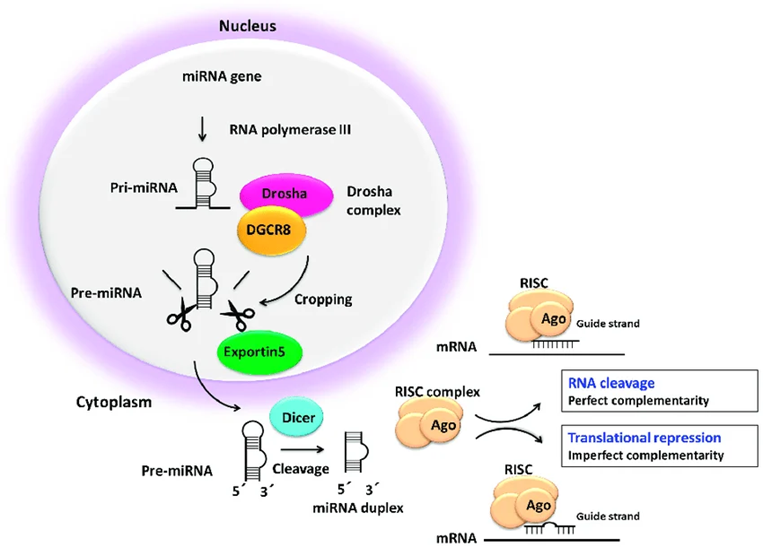
\includegraphics[width=\textwidth]{figures/image.png}
\end{columns}
\vfill
\scriptsize Factors Regulating microRNA Expression and Function in Multiple Myeloma -- Scientific Figure on ResearchGate. Available from: \url{https://www.researchgate.net/figure/miRNA-biogenesis-pathway-RISC-RNA-induced-silencing-complex-Ago-Argonaute-family_fig1_330472148} [accessed 15 Apr 2026]
\end{frame}

\begin{frame}{Binding des miRNA par le seed}
\begin{columns}[T, onlytextwidth]
	\column{0.45\textwidth}
	\begin{itemize}\setlength\itemsep{1em}
		\item Seed
		\item Bridge (central / unpaired)
		\item Supplementary
		\item Tail
	\end{itemize}

	\column{0.5\textwidth}
	\centering
	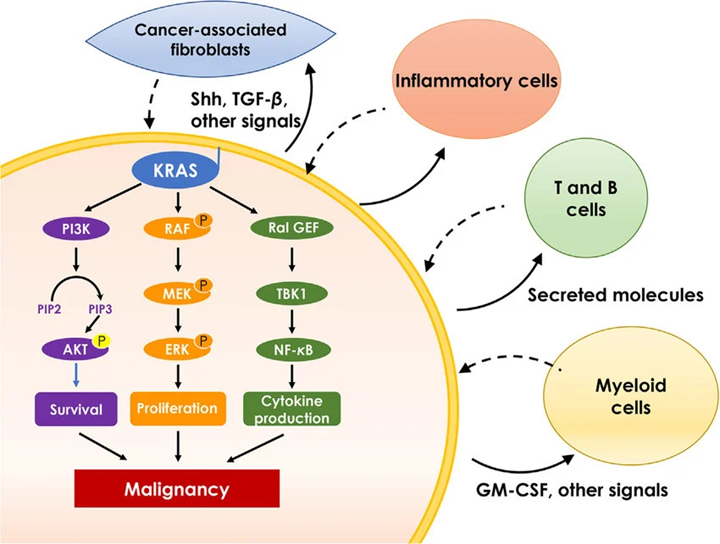
\includegraphics[width=\textwidth]{figures/image3.png}
\end{columns}
\vfill
\scriptsize Garg, A., Braviner, L., Axhemi, A., Bibel, B., \& Joshua-Tor, L. (2026). Structural dynamics between Argonaute-2 and CK1$\alpha$ promote target RNA release in microRNA-mediated silencing. \textit{bioRxiv}. \url{https://doi.org/10.64898/2026.03.23.713669}
\end{frame}

\begin{frame}{Pourquoi le réseau KRAS}
\begin{columns}[T, onlytextwidth]
	\column{0.45\textwidth}
	\begin{itemize}\setlength\itemsep{1em}
		\item Présent dans plusieurs cancers
		\item Réseau complexe avec beaucoup d'interactions possible avec les miRNA
		\item La protéine KRas est résistante aux approches classiques donc les miRNA sont une approche qui a du potentiel
	\end{itemize}

	\column{0.5\textwidth}
	\centering
	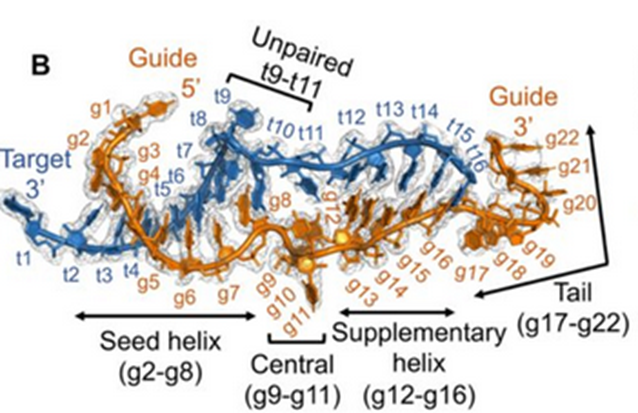
\includegraphics[width=\textwidth]{figures/image2.png}
\end{columns}
\vfill
\scriptsize Targeting the untargetable KRAS in cancer therapy -- Scientific Figure on ResearchGate. Available from: \url{https://www.researchgate.net/figure/The-major-KRAS-effector-pathways-Oncogenic-KRAS-activates-intracellular-PI3K-MAPK-or_fig1_331568339} [accessed 16 Apr 2026]
\end{frame}

\begin{frame}{Database Gencode v46}
\begin{columns}[T, onlytextwidth]
	\column{0.45\textwidth}
	\begin{itemize}\setlength\itemsep{1em}
		\item Database des éléments fonctionnels du génome humain
		\item Basé sur le génome GRCh38.p14
		\item La database utilisée par RIMap-RISC
	\end{itemize}

	\column{0.5\textwidth}
	\centering
	
\includegraphics[width=\textwidth]{figures/image4.png}
\end{columns}
\end{frame}
